\documentclass{beamer}

\usepackage[utf8]{inputenc}
\usepackage[english]{babel}
\usepackage{default}
\usepackage{graphicx}
\usepackage{caption}
\usepackage{xcolor}

\usetheme{Rochester}
\usecolortheme{default}


\author{Till Fastnacht}
\title{Visualisierung - Abschlussprojekt}
\subtitle{Vergleich von Wetterdaten}
\date{2015/12/16}
\institute{Bauhaus-Universität Weimar}

% comment

\begin{document}

  \begin{frame}
  \titlepage
  \end{frame}
  
  \begin{frame}
  \frametitle{Daten}
    \begin{columns}
      \column{0.5\textwidth}
	\begin{itemize}
	  \item Daten aus Jena (Station Max-Planck Institut für Bio-Geochemie)
	  \item Messung alle 10min seit 2004
	  \begin{itemize}
	    \item Datum und Zeit des Datensatzes (Ende)
	    \item Luftdruck
	    \item Lufttemperatur
	    \item relative Luftfeuchte
	    \item Windgeschwindigkeit
	    \item Niederschlag
	  \end{itemize}
	\end{itemize}
      \column{0.5\textwidth}
	\begin{figure}[h]
	\centering
	    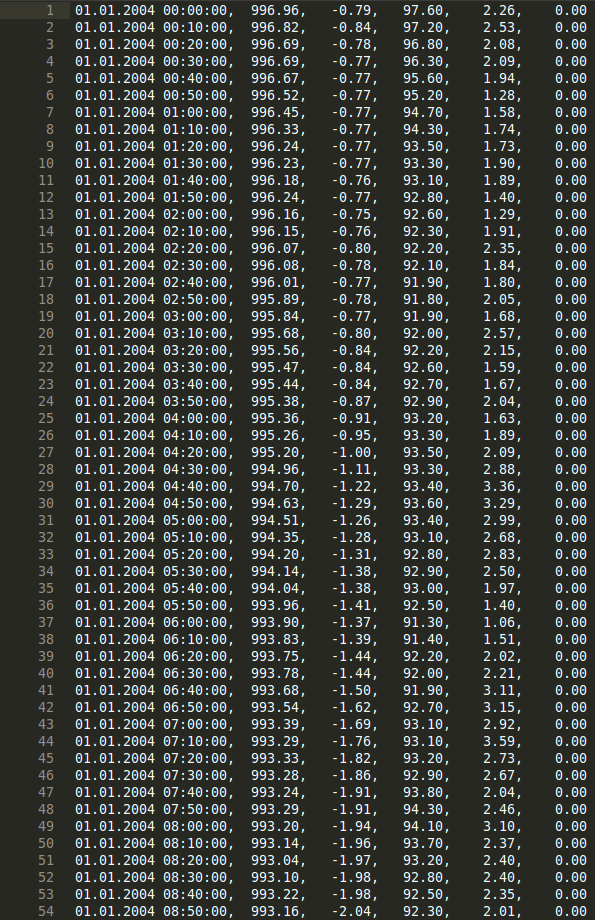
\includegraphics[width=.3\paperwidth,keepaspectratio=true]{./media/data.png}
	    % Screenshot from 2015-12-15 19:29:36.png: 0x0 pixel, 300dpi, 0.00x0.00 cm, bb=
	\end{figure}
   \end{columns}
  \end{frame} 
  
  \begin{frame}
   \frametitle{Idee}
   \begin{block}{erste Idee...}
    ...die Daten so aufarbeiten und darstellen, dass man die Möglichkeit hat Tage und Jahre miteinander zu vergleichen
   \end{block}

  \end{frame}


  \begin{frame}
  \frametitle{Ziel 1/6 - Detail}
    \begin{itemize}
      \item Informationen über einen Tage in einem Jahr erlangen
      \visible<2->{
	\begin{itemize}
	  \item zBsp Luftfeuchte am 18. Juli 2004
	\end{itemize}
      }
      \visible<3->{
      \begin{figure}[h]
	\centering
	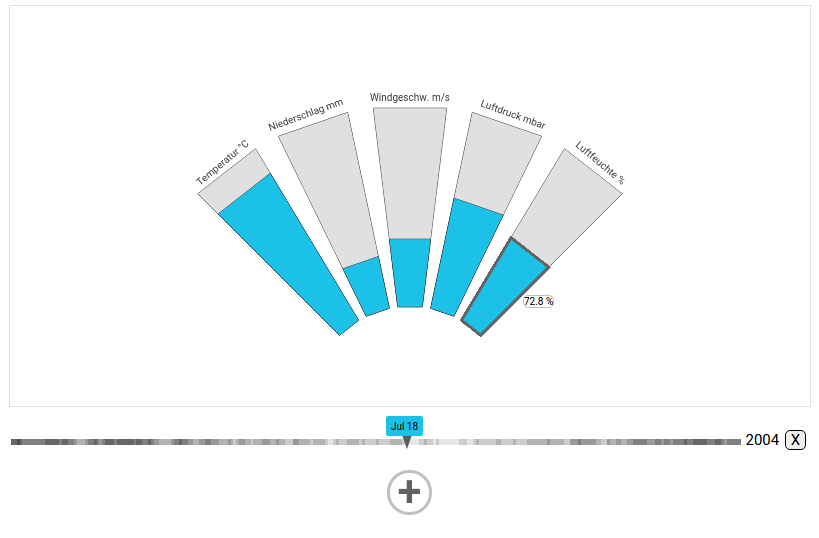
\includegraphics[width=.5\paperwidth,keepaspectratio=true]{./media/one_year.png}
	    % Screenshot from 2015-12-15 19:29:36.png: 0x0 pixel, 300dpi, 0.00x0.00 cm, bb=
	\end{figure}
      }
    \end{itemize}
  \end{frame}  
  
  \begin{frame}
  \frametitle{Ziel 2/6 - Detail}
    \begin{itemize}
      \item Daten gleicher Tage verschiedener Jahre vergleichen
      \visible<2->{
	\begin{itemize}
	  \item zBsp Windgeschwindigkeit 11. April 2004 und 2008
	\end{itemize}
      }
      \visible<3->{
      \begin{figure}[h]
	\centering
	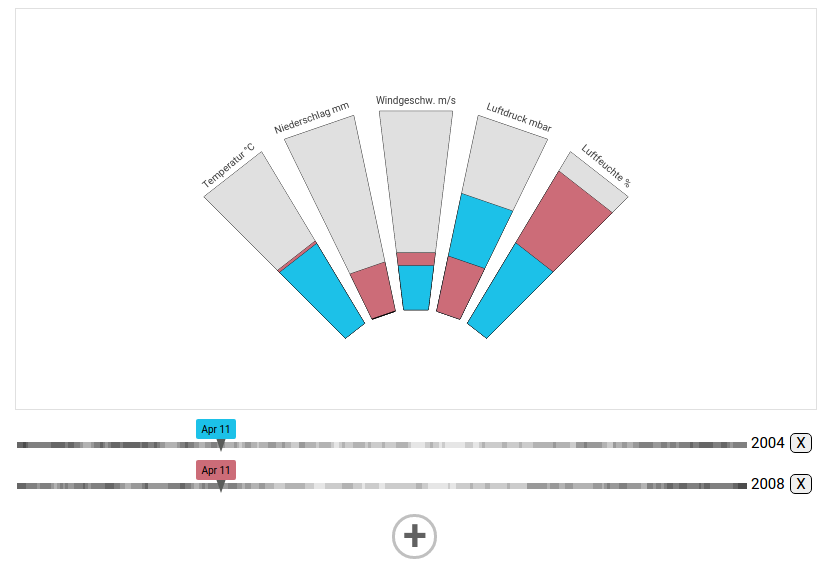
\includegraphics[width=.5\paperwidth,keepaspectratio=true]{./media/two_years_same_day.png}
	    % Screenshot from 2015-12-15 19:29:36.png: 0x0 pixel, 300dpi, 0.00x0.00 cm, bb=
	\end{figure}
      }
    \end{itemize}
  \end{frame}
  
  \begin{frame}
  \frametitle{Ziel 3/6 - Detail}
    \begin{itemize}
      \item Daten unterschiedlicher Tage verschiedener Jahre vergleichen
      \visible<2->{
	\begin{itemize}
	  \item zBsp Temperatur 2. Mai 2004 und 13. Oktober 2008
	\end{itemize}
      }
      \visible<3->{
      \begin{figure}[h]
	\centering
	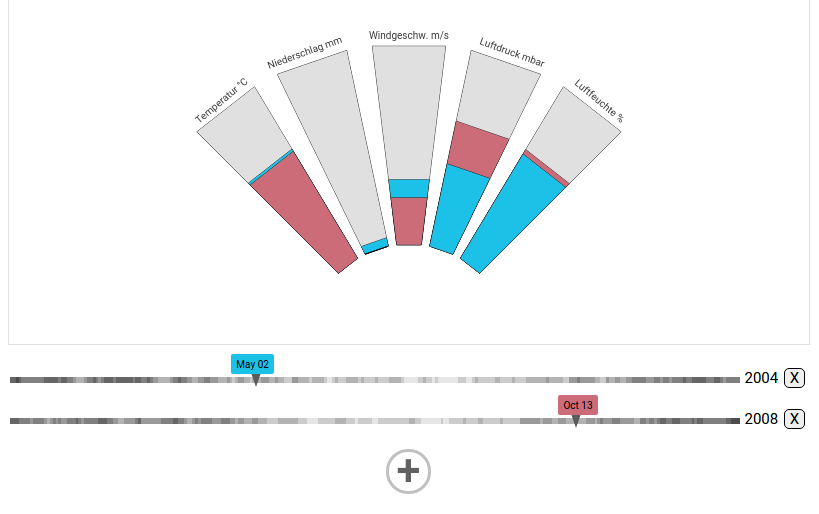
\includegraphics[width=.5\paperwidth,keepaspectratio=true]{./media/two_year_different_day.png}
	    % Screenshot from 2015-12-15 19:29:36.png: 0x0 pixel, 300dpi, 0.00x0.00 cm, bb=
	\end{figure}
      }
    \end{itemize}
  \end{frame}
  
  \begin{frame}
  \frametitle{Ziel 4/6 - Overview}
    \begin{itemize}
      \item eine Jahresübersicht über einen ausgewählten Datentyp haben
      \visible<2->{
	\begin{itemize}
	  \item zBsp Niederschlag des Jahres 2004 plotten
	\end{itemize}
      }
      \visible<3->{
      \begin{figure}[h]
	\centering
	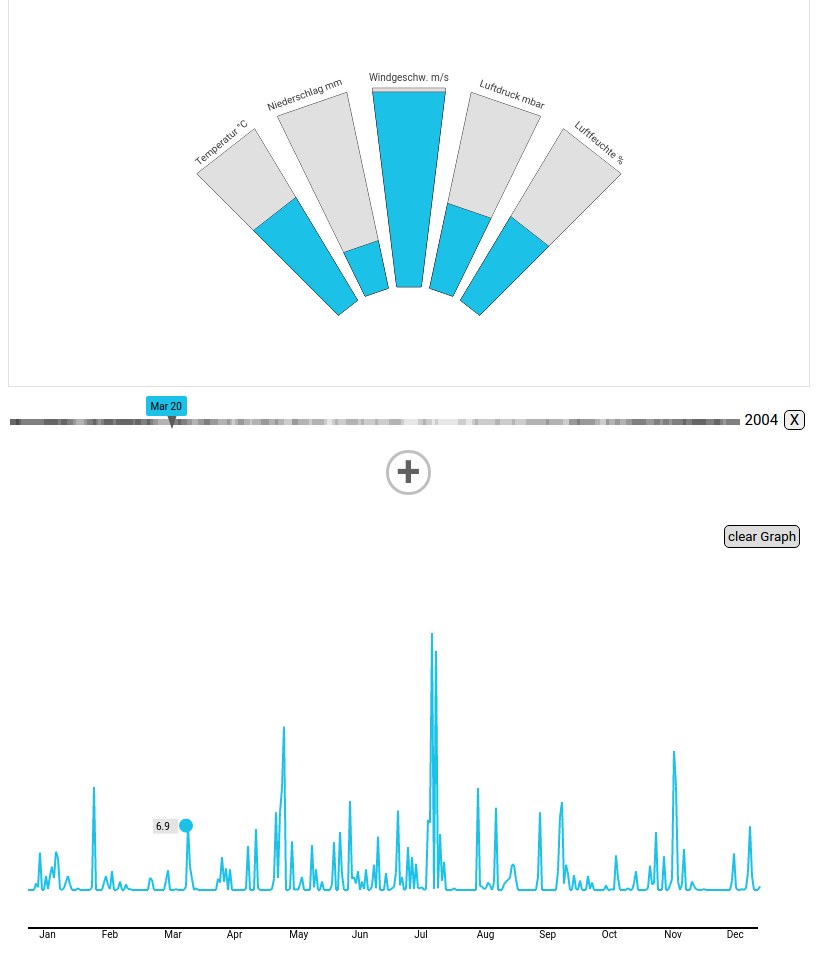
\includegraphics[width=.4\paperwidth,keepaspectratio=true]{./media/graph_one_year_rain.png}
	    % Screenshot from 2015-12-15 19:29:36.png: 0x0 pixel, 300dpi, 0.00x0.00 cm, bb=
	\end{figure}
      }
    \end{itemize}
  \end{frame}
  
  \begin{frame}
  \frametitle{Ziel 5/6 - Overview}
    \begin{itemize}
      \item eine Jahresübersicht über mehrere ausgewählten Datentyp haben
      \visible<2->{
	\begin{itemize}
	  \item zBsp Niederschlag und Temperatur des Jahres 2004 plotten
	\end{itemize}
      }
      \visible<3->{
      \begin{figure}[h]
	\centering
	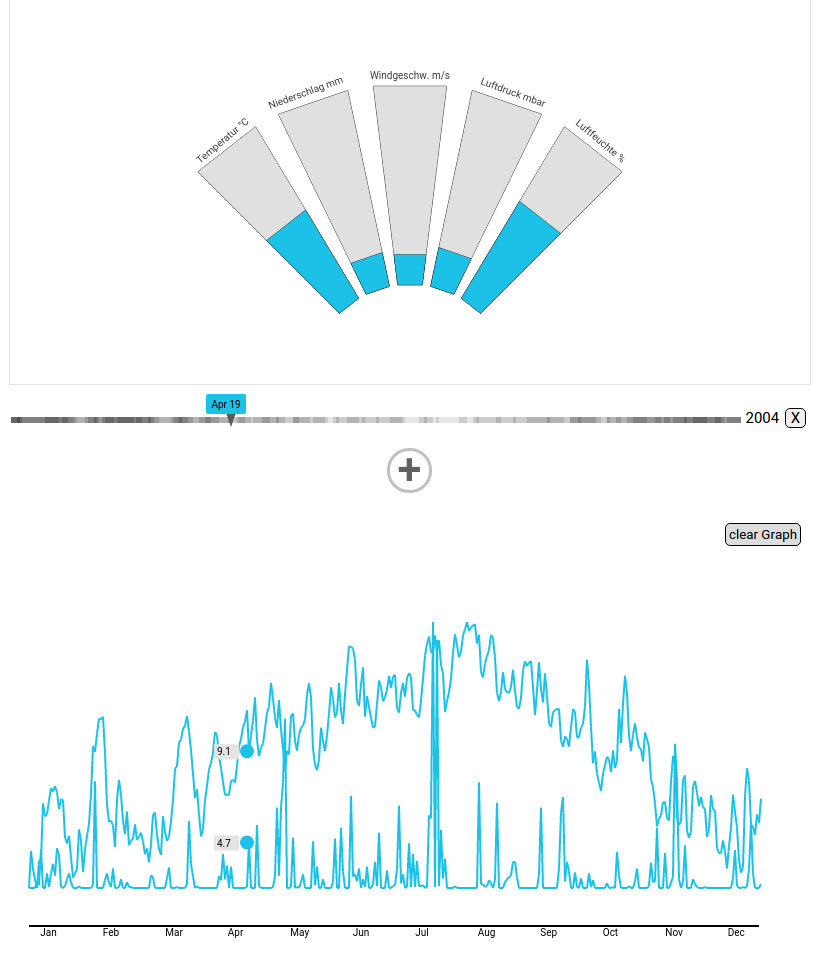
\includegraphics[width=.4\paperwidth,keepaspectratio=true]{./media/graph_one_year_two_data.png}
	    % Screenshot from 2015-12-15 19:29:36.png: 0x0 pixel, 300dpi, 0.00x0.00 cm, bb=
	\end{figure}
      }
    \end{itemize}
  \end{frame}
  
  \begin{frame}
  \frametitle{Ziel 6/6 - Overview}
    \begin{itemize}
      \item gleiche Daten im Verlauf eines Jahres ansehen können
      \visible<2->{
	\begin{itemize}
	  \item zBsp Temperatur des Jahres 2004 und 2008 plotten
	\end{itemize}
      }
      \visible<3->{
      \begin{figure}[h]
	\centering
	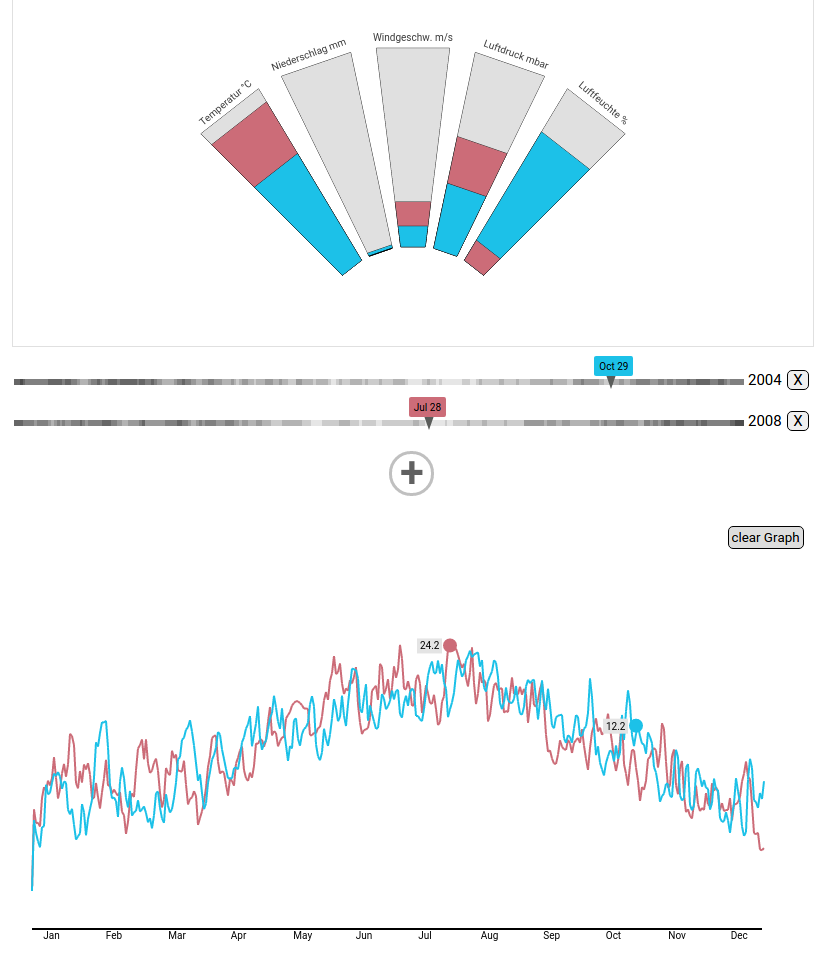
\includegraphics[width=.4\paperwidth,keepaspectratio=true]{./media/graph_two_years_temp.png}
	    % Screenshot from 2015-12-15 19:29:36.png: 0x0 pixel, 300dpi, 0.00x0.00 cm, bb=
	\end{figure}
      }
    \end{itemize}
  \end{frame}

  \begin{frame}
  \frametitle{Funktionalität}
  \begin{itemize}
    \item beliebig Jahre hinzufügen und entfernen (selection)
    \item unabhängig Details einzelner Tage anzeigen (navigation, change)
    \item Übersicht über den Verlauf der Temperatur eines Jahres anhand Grauwerten im Slider
    \item Graphen in Abhängigkeit anzeigen lassen:
    \begin{itemize}
      \item verschiedener Datentyp von einem Jahr 
      \\ oder
      \item gleicher Datentyp von mehreren Jahren
    \end{itemize}

  \end{itemize}

  \end{frame}

  
  \begin{frame}
  \frametitle{WHAT}
    \begin{itemize}
    \item Dataset Type
      \begin{itemize}
	  \item Table 
	  \begin{itemize}
	   \item Attribute: Temperatur, Niederschlag, ...
	   \item Item: Attribute zu einem gewissen Zeitpunkt
	  \end{itemize}
      \end{itemize}
    \item Attribute Type
      \begin{itemize}
	\item geordnet $\rightarrow$ quantitative
	\item zBsp Temperatur, Luftfeuchte, ...
      \end{itemize}
    \item Dataset Availability
      \begin{itemize}
	\item static (10 Jahre)
      \end{itemize}
    \end{itemize}  
  \end{frame} 
  
  \begin{frame}
  \frametitle{WHY}
  $\rightarrow$ vgl. ``Ziele''
    \begin{itemize}
      \item \{action : target\}
      \item present : distribution
      \item locate : extremes
      \item compare : similarity
      \item compare : correlation
    \end{itemize}
  \end{frame}
  
  \begin{frame}
  \frametitle{HOW - Encode}
    \begin{itemize}
      \item \textbf{marks}
	\begin{itemize}
	  \item area (Detailansicht)
	  \item lines (Graphen, Slider)
	\end{itemize}
      \item \textbf{channels}
	\begin{itemize}
	  \item bars
	  \begin{itemize}
	   \item shape (min - max)
	   \item size (area)
	   \item color (year)
	  \end{itemize}
	  \item slider
	  \begin{itemize}
	   \item color (temperature overview)
	  \end{itemize}
	  \item graphs
	  \begin{itemize}
	   \item color(year)
	  \end{itemize}
	\end{itemize}
    \end{itemize}
  \end{frame}
  
  \begin{frame}
  \frametitle{HOW - Manipulate}
    \textbf{detail + overview}
    \begin{figure}[h]
      \centering
      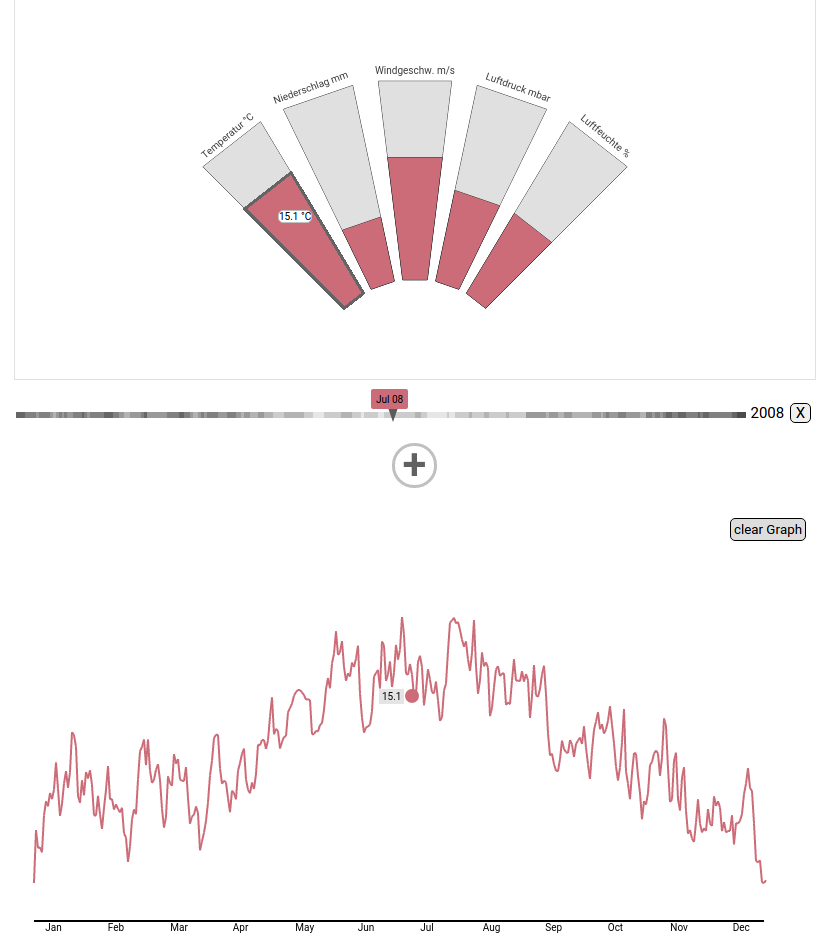
\includegraphics[width=.4\paperwidth,keepaspectratio=true]{./media/overview_detail.png}
      % Screenshot from 2015-12-15 19:29:36.png: 0x0 pixel, 300dpi, 0.00x0.00 cm, bb=
    \end{figure}
  \end{frame}
  
  \begin{frame}
  \frametitle{HOW - Facet}
    \textbf{brushing \& linking}
    \begin{itemize}
     \item Farbe von
     \begin{itemize}
      \item Detailansicht
      \item Slider Thumbnail
      \item Linie Graph
     \end{itemize}
     \item Hervorhebung im Graph - Position Slider
     \end{itemize}
    \begin{figure}[h]
      \centering
      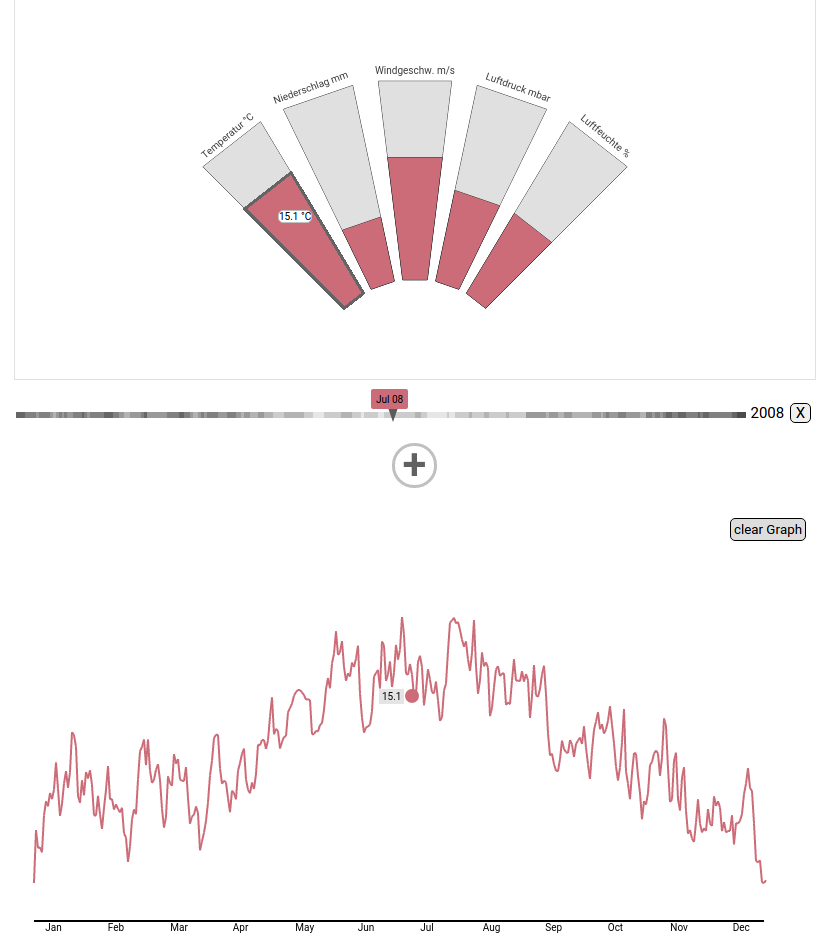
\includegraphics[width=.3\paperwidth,keepaspectratio=true]{./media/overview_detail.png}
      % Screenshot from 2015-12-15 19:29:36.png: 0x0 pixel, 300dpi, 0.00x0.00 cm, bb=
    \end{figure}
  \end{frame}

  \begin{frame}
  \frametitle{HOW - Facet}
    \textbf{superimpose}
    \begin{itemize}
     \item Überlagerung von:
     \begin{itemize}
      \item Daten in Detailansicht (kleinster Wert im Vordergrund - keine Verdeckung)
      \item Graphen
     \end{itemize}
    \end{itemize}
    \begin{figure}[h]
      \centering
      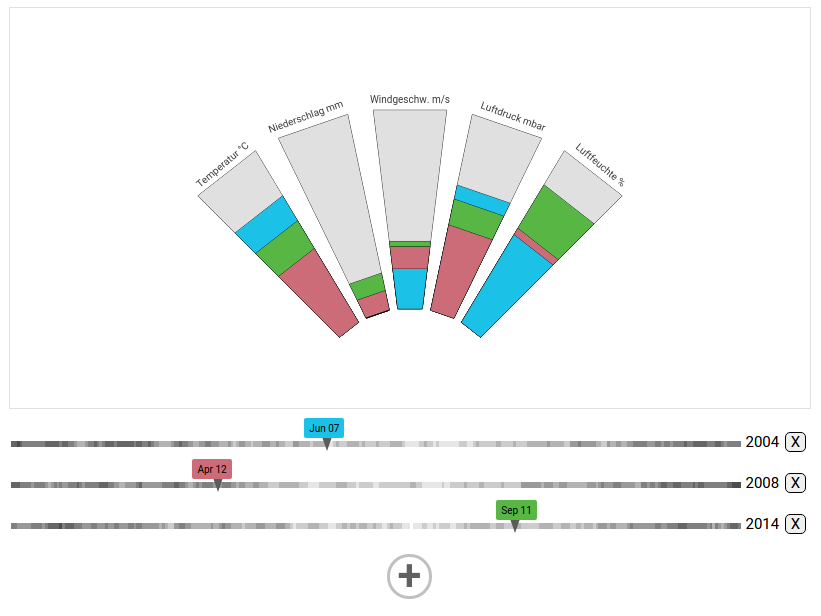
\includegraphics[width=.4\paperwidth,keepaspectratio=true]{./media/superimpose.png}
      % Screenshot from 2015-12-15 19:29:36.png: 0x0 pixel, 300dpi, 0.00x0.00 cm, bb=
    \end{figure}
  \end{frame}

  \begin{frame}
  \frametitle{HOW - Reduce}
    \textbf{detail on demand}
    \\ focus \& context
    \\ bei MouseOver werden mehr Informationen/genauer Wert mit Einheit angezeigt
    \begin{figure}[h]
      \centering
      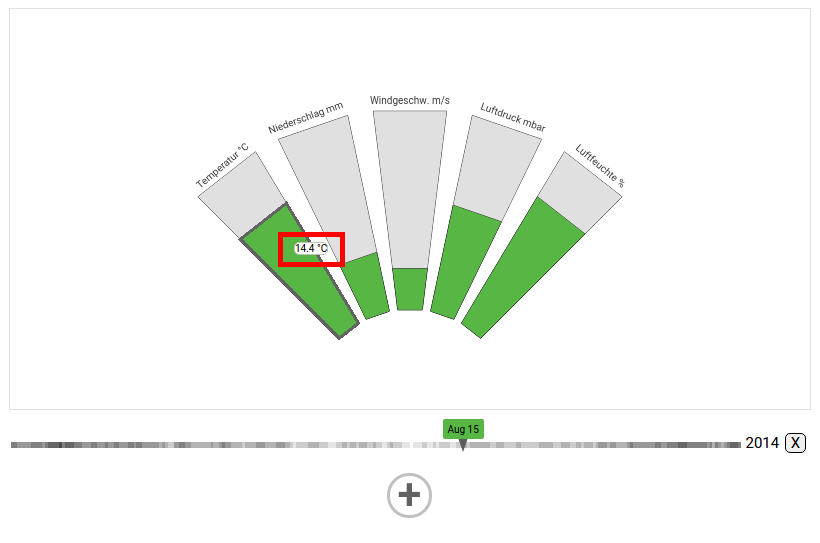
\includegraphics[width=.6\paperwidth,keepaspectratio=true]{./media/detail_on_demand.png}
      % Screenshot from 2015-12-15 19:29:36.png: 0x0 pixel, 300dpi, 0.00x0.00 cm, bb=
    \end{figure}
  \end{frame}
  
  \begin{frame}
  \centering
  Vielen Dank für Ihre Aufmerksamkeit
  \end{frame}



  
\end{document}

